\chapter{Simulation Domains and Meshes}\label{chap:mesh}
\section{Generating meshes}\label{sec:meshGeneration}
A simulation begins with a mesh file describing the specimen geometry, volume elements and region IDs. Simple specimens can be generated with \href{https://gmsh.info/}{Gmsh}; more elaborate polycrystalline specimens can be generated with \href{https://neper.info/}{Neper}. After generation, MoDELib reads the mesh and constructs the connectivity and grain-boundary topology used by the simulation.

\subsection{Simple geometries with Gmsh}
Gmsh provides geometry definition and finite-element mesh generation. For cubes, cylinders and simple partitions, start from the geometry files \code{Library/Meshes/unitCube.geo}, \code{cylinder.geo} or \code{bicrystal.geo}. For example, from the repository root:
\begin{lstlisting}[language=bash,basicstyle=\footnotesize\ttfamily]
gmsh Library/Meshes/unitCube.geo -3 -order 1 -format msh2 -o mesh.msh
\end{lstlisting}
This writes a tetrahedral mesh to \code{mesh.msh}; changing the geometry's size parameters changes the discretization. The current reader uses ASCII Gmsh version 2 records and takes the second element tag as the region ID. Preserve distinct volume entities for different grains. See the \href{https://gmsh.info/doc/texinfo/gmsh.html}{Gmsh reference manual} for geometry and meshing options.

\subsection{Polycrystals and periodicity with Neper}
Neper generates grain tessellations and meshes them, including periodic and partially periodic polycrystals. Its tessellation and meshing stages are separate:
\begin{lstlisting}[language=bash,basicstyle=\footnotesize\ttfamily]
neper -T -n 10 -periodicity all -o poly10
neper -M poly10.tess -order 1 -format msh:ascii
\end{lstlisting}
These commands illustrate a ten-grain periodic tessellation and its mesh; they are not recipes for reproducing a particular stored library file. Neper's meshing stage uses Gmsh for tetrahedral meshing. The \href{https://neper.info/doc/neper_t.html}{tessellation documentation} describes grain morphology and periodicity, and the \href{https://neper.info/doc/neper_m.html}{meshing documentation} describes element size and output formats.

Neper's periodicity selector accepts all directions or a subset of its generation axes, such as \code{x,y}. Periodic directions in the simulation need not align with the global Cartesian axes: rotate a periodic mesh into the desired frame, or apply the nonsingular import transformation $\bm F$ introduced below. A source translation $\bm a_k$ then becomes $\bm F\bm a_k$, allowing oblique directions as well. The same transformation must act on the whole mesh so that paired nodes and triangulations still match. MoDELib activates the desired geometric pairing when the mesh is constructed; generating a periodic file alone does not select a field boundary condition.

\subsection{Examples in the mesh library}
Figure~\ref{fig:meshLibrary} shows four existing files from \code{Library/Meshes}. The cube and cylinder provide single-region examples; the bicrystal introduces a grain boundary. The ten-grain periodic unit has a jagged exterior following whole grains, and translated copies fill space. Its exterior is not a cut through grains at the boundary of a rectangular box.
\begin{figure}[t]
\centering
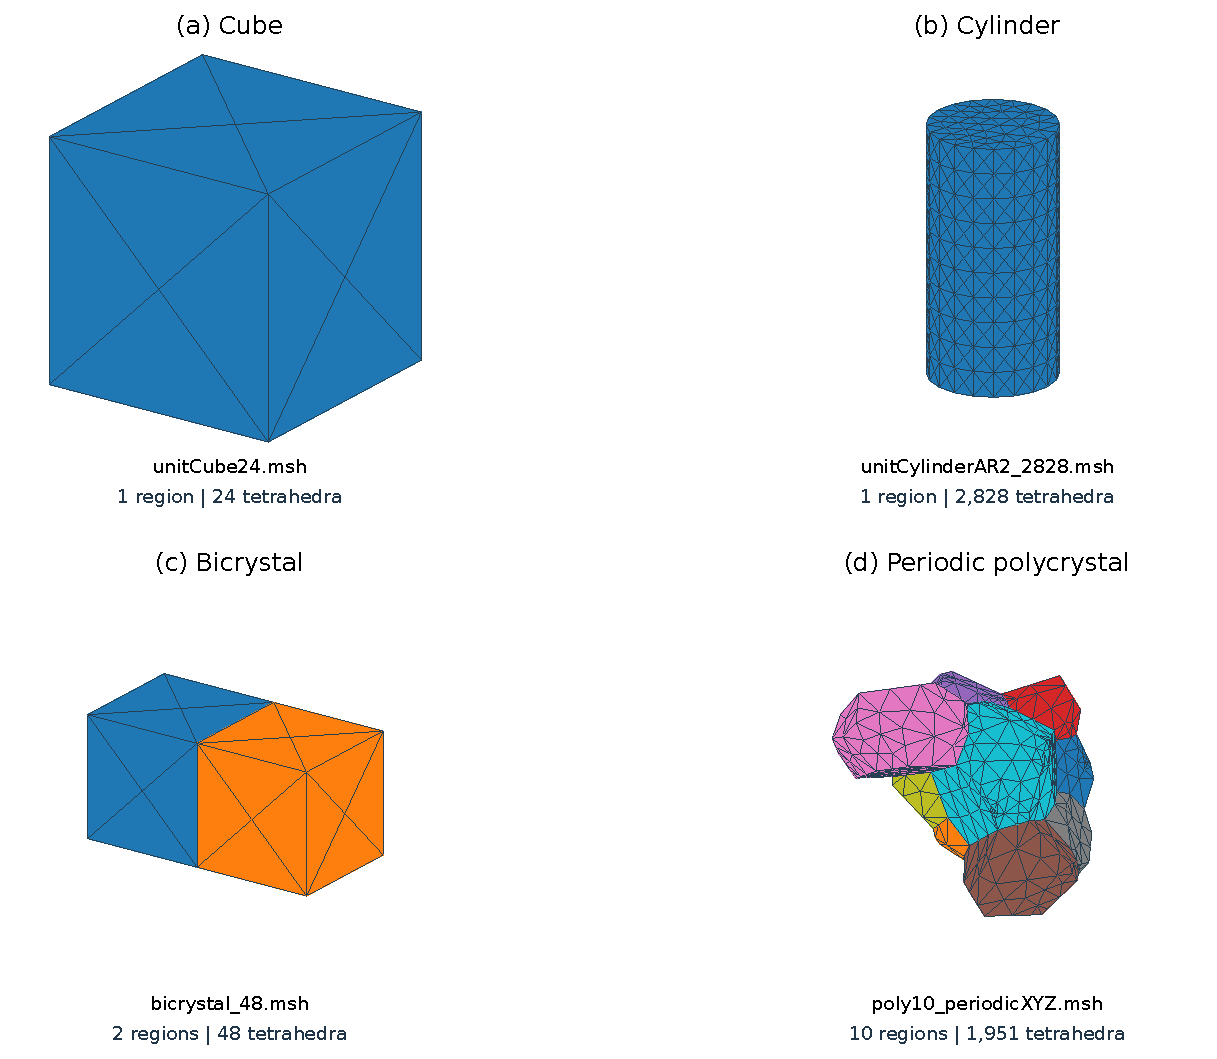
\includegraphics[width=0.98\textwidth]{mesh_library_examples}
\caption{Existing volume meshes in \code{Library/Meshes}, displayed through their exterior triangulations. Colors identify region IDs. Each specimen is scaled independently for display; counts refer to volume tetrahedra. Quadratic edge nodes, when present in the source file, are omitted from the sketches.}\label{fig:meshLibrary}
\end{figure}
Further examples include \code{polycrystalCube_10_periodicX.msh}, \code{polycrystalCube_10_periodicXY.msh}, \code{poly30_periodicXYZ.msh} and \code{polycrystalCyl_50.msh}. Select a file with the geometry, grain structure and matching periodic boundaries required by the problem, then check its region IDs against the material input.
\sourcefile{src/Mesh/SimplexReader.cpp}


\clearpage
\section{MoDELib mesh architecture}\label{sec:meshArchitecture}
The \code{.msh} mesh files are the input to the MoDELib mesh representation. The mesh constructor reads coordinates and connectivity, applies the prescribed transformation, and inserts the volume elements.

\subsection{Constructing a mesh from a file}
Both examples load \code{mesh.msh} from the working directory with the identity transformation, zero origin shift and no periodic face pairing. The coordinates are mapped as $\bm x=\bm F(\bm X-\bm x_0)$. Replace the filename with your mesh path. C++ requires MoDELib's include and link settings; Python requires NumPy and an importable \code{pyMoDELib} module.

\noindent\begin{minipage}{\linewidth}
\begin{minipage}[t]{0.48\linewidth}
\begin{tcolorbox}[enhanced,colback=manualblue!5,colframe=manualblue!35,boxrule=0.4pt,
 arc=1mm,left=2mm,right=2mm,top=7mm,bottom=2mm,height=5cm,
 overlay={\node[anchor=north east,inner sep=1mm] at (frame.north east) {\cppsymbol};}]
\begin{lstlisting}[language=C++,basicstyle=\footnotesize\ttfamily,frame=none,backgroundcolor=\color{manualblue!5},aboveskip=0pt,belowskip=0pt]
#include <MeshModule.h>

int main()
{
    Eigen::Matrix3d F = // deformation gradient
        Eigen::Matrix3d::Identity();
    Eigen::Vector3d x0 = // origin shift
        Eigen::Vector3d::Zero();

    model::SimplicialMesh<3> mesh(
        "mesh.msh", F, x0, {});
}
\end{lstlisting}
\end{tcolorbox}
\end{minipage}\hfill
\begin{minipage}[t]{0.48\linewidth}
\begin{tcolorbox}[enhanced,colback=Goldenrod!9,colframe=Goldenrod!55!black,boxrule=0.4pt,
 arc=1mm,left=2mm,right=2mm,top=7mm,bottom=2mm,height=5cm,
 overlay={\node[anchor=north east,inner sep=2mm] at (frame.north east) {\pythonsymbol};}]
\begin{lstlisting}[language=Python,basicstyle=\footnotesize\ttfamily,frame=none,backgroundcolor=\color{Goldenrod!9},aboveskip=0pt,belowskip=0pt]
import numpy as np
import pyMoDELib

F = np.eye(3)     # deformation gradient
x0 = np.zeros(3)  # origin shift

mesh = pyMoDELib.SimplicialMesh3(
    "mesh.msh", A=F, x0=x0,
    periodicFaceIDs=set()
)
\end{lstlisting}
\end{tcolorbox}
\end{minipage}
\captionsetup{hypcap=false}
\captionof{lstlisting}{Creating a mesh.}
\end{minipage}
\sourcefile{tools/pyMoDELib/MeshBindingsImplementation.h}


\subsection{Simplicial and polyhedral representations}
MoDELib implements both a discretization of the material volume and a description of its boundary topology:
\begin{itemize}
\item \code{SimplicialMesh<dim>} stores volume simplices and their lower-dimensional children. In three dimensions, these are tetrahedra, triangles, edges and vertices. It provides global point search functions and supports the finite-element architecture described in Section~\ref{sec:femArchitecture}.
\item \code{PolyhedralMesh<dim>} stores a cell complex of the grains: regions, planar faces, perimeter edges and vertices. It supports oriented boundary traversal and plane sections.

A polyhedral region is a grain-shaped volume bounded by faces. Similarly, a polyhedral face may contain many triangular mesh faces. Internal triangulation edges are absent from its perimeter, while subdivisions of the perimeter, including collinear mesh vertices, are retained.
\end{itemize}

The two representations therefore share geometry without assigning the same meaning to every edge or face.
\begin{figure}[t]
\centering
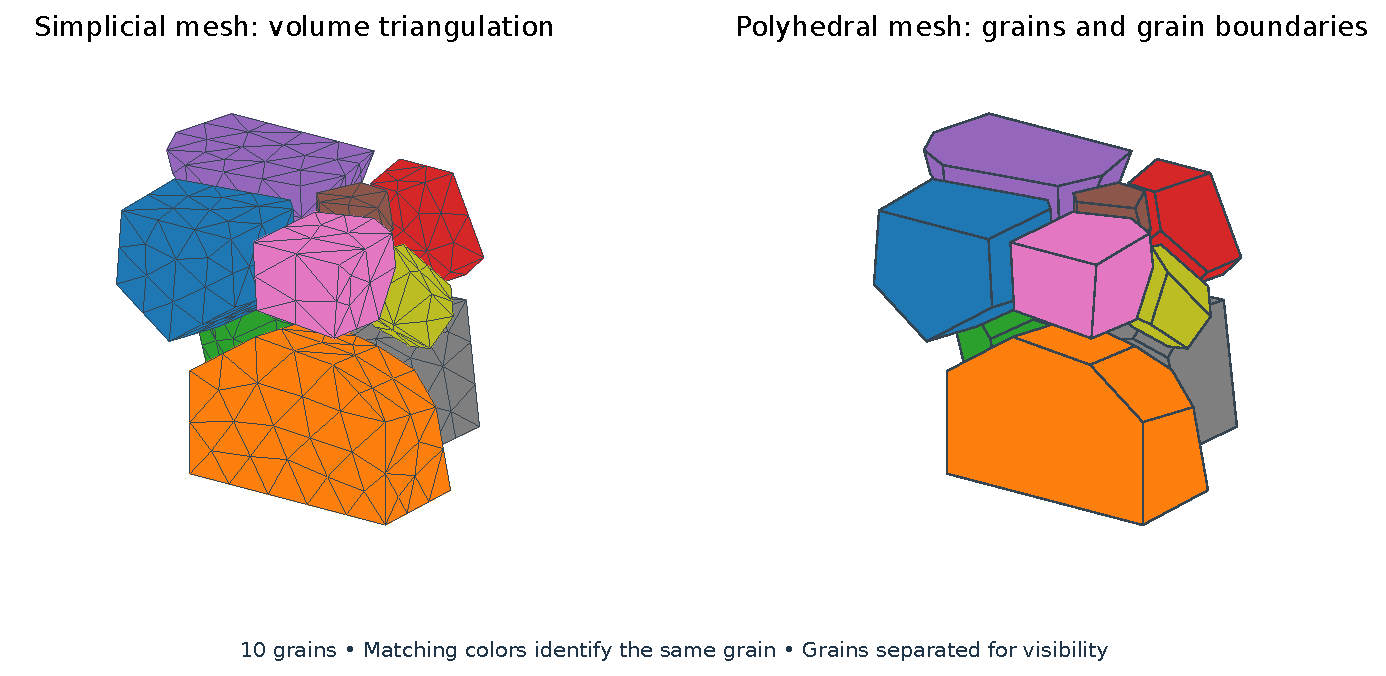
\includegraphics[width=0.80\textwidth]{polycrystal_mesh_views}
\caption{Two views of the ten-grain mesh \code{Library/Meshes/polycrystalCube_10_periodicX.msh}, containing 1081 tetrahedra. Left: the boundary triangulation of each grain, shown using tetrahedron corner vertices; quadratic edge nodes are omitted. Right: the same grain faces with internal coplanar triangle edges suppressed. Colors identify corresponding grains. Grains are separated only for visualization, exposing internal interfaces.}
\end{figure}
\sourcefile{include/Mesh/SimplicialMesh.h}
\sourcefile{include/Mesh/PolyhedralMesh.h}

\section{Simplices and shared topology}
A \code{Simplex<dim,order>} represents a simplex of topological dimension \code{order}. Vertex IDs define its identity; adjacent higher-order simplices share lower-order entities. The mesh indexes entities through one \code{SimplexFactory<dim,order>} per order, accessed with \code{simplexFactory<order>()}. The factory canonicalizes the vertex-ID key and reuses an existing simplex through \code{getOrCreate}; the same volume simplex cannot be assigned to two regions.

The mesh's \code{simplices()} map owns the volume simplices. Each simplex owns its children through shared pointers, while child-to-parent links and factory entries are weak pointers. \code{liveSimplices()} returns a map of shared pointers to the currently live entities; \code{parents()} similarly returns a temporary map of live parents. Use these views for traversal rather than treating raw factory entries as owning pointers. \code{pruneExpired()} removes expired factory entries. Keep the mesh alive while using its entities, since they also refer to mesh-owned geometry and factories.
\sourcefile{include/Mesh/SimplexFactory.h}
\sourcefile{include/Mesh/SimplexChild.h}
\sourcefile{include/Mesh/SimplexParent.h}
\manualfigure{simplex_complex}{0.98}{The simplex hierarchy in three dimensions. Arrows lead to lower-dimensional boundary entities; orange highlights a selected child in each sketch. Dashed lines show the tetrahedron's hidden edges.}

For a point $\bm x$, a tetrahedron's barycentric coordinates satisfy
\begin{equation}
\bm x=\sum_{a=0}^{3}\lambda_a\bm X_a,\qquad
\sum_{a=0}^{3}\lambda_a=1.
\end{equation}
Nonnegative coordinates characterize containment, up to numerical tolerance. The C++ search routines return a success flag and a simplex pointer. Check the flag before using the pointer as a containing element. \code{searchWithGuess} permits reuse of a nearby element, while \code{searchRegion} and \code{searchRegionWithGuess} restrict the search to a grain. This distinction is important near an interface, where geometry alone does not select a unique crystal orientation. In Python, \code{mesh.search(point)} returns the containing simplex on success and \code{None} on failure; it does not return the C++ pair.
\sourcefile{src/Mesh/SimplicialMesh.cpp}

\section{Polyhedral cells and oriented incidence}
\code{Polyhedron<dim,order>} is the common cell type. In three dimensions, a region is order 3, a face order 2, an edge order 1 and a vertex order 0. One factory per order provides shared entities keyed by IDs. Regions and faces use scalar region and face IDs as keys; lower-dimensional boundary cells are keyed by their vertex IDs.

Region cells, \code{Polyhedron<dim,dim>}, group volume simplices by region ID. A boundary between two regions is represented by \code{MeshRegionBoundary}; its planar pieces are codimension-one \code{Polyhedron<dim,dim-1>} objects.

The mesh constructor then constructs region boundaries, updates regions and their planar faces in the shared polyhedral factories, completes their boundary topology, and finally identifies active periodic face pairs. This order matters: periodic matching operates on completed external faces, and downstream consumers must see a consistent topology.

Children are held by shared pointers and parents by weak pointers. This allows a face to belong to two regions, or an edge to several faces, without creating parent--child ownership cycles. Each cell also stores its associated simplices. Codimension-one cells carry face normals, centers, region IDs and periodic partners directly. This unified representation replaces the earlier separate \code{MeshRegion} and \code{PlanarMeshFace} classes in the current mesh refactor. In 3D, a face with one incident region is external; a face with two incident regions separates grains.
\manualfigure{cell_complex}{0.98}{Geometric entities of the polyhedral complex in three dimensions. Orange highlights a selected child in each sketch. Blue arrows point to children (shared ownership); orange arrows point to parents (weak references). A face can belong to two regions. The polygonal prism is illustrative; grains may have more general shapes.}

An edge itself has no single orientation valid for every face. \code{PolyhedralFaceIncidence} supplies the orientation of that edge within one face perimeter through its \code{reversed} flag and perimeter index. \code{source()}, \code{sink()} and \code{tangent()} use that orientation. \code{next()} and \code{prev()} traverse the same perimeter; in 3D, \code{otherFace(regionID)} crosses the edge to the adjacent face bounding the specified region. Specifying the region is essential at a grain junction, where an edge can have more than two parent faces.

The constructor derives boundaries by counting simplex incidences. A boundary sub-simplex occurs once; an internal one occurs twice. Validation rejects duplicate or non-manifold input, branched or disconnected edges, and open, repeated or multiple polygon perimeters. The current polygon representation requires one closed perimeter per 2-cell; do not assume support for a face with holes. Normal orientation and grain-shell checks have a specialized 3D implementation.
\sourcefile{include/Mesh/PolyhedralMeshImplementation.h}
\sourcefile{src/Mesh/PolyhedralMesh.cpp}

\section{Mesh access from Python}
The bindings expose \code{SimplicialMesh1}, \code{SimplicialMesh2} and \code{SimplicialMesh3}, with corresponding \code{SimplexReader1/2/3} and \code{PolyhedralMesh1/2/3} types. \code{SimplicialMesh} and \code{SimplexReader} remain aliases for the three-dimensional types. Entity names encode dimension and order: for example, \code{Simplex32} is a triangular simplex in 3D and \code{Polyhedron32} is a polyhedral face in 3D. The older \code{Polyhedron0/1/2/3} names alias the corresponding 3D entities.

The Python mesh constructor accepts \code{filename}, \code{A}, \code{x0} and \code{periodicFaceIDs}. The last three arguments default to the identity matrix, zero vector and empty set, so \code{SimplicialMesh3("mesh.msh")} is sufficient for an untransformed, nonperiodic mesh. A \code{SimplexReader3} can instead read coordinates and connectivity without constructing mesh topology: \code{reader.read(filename)}, \code{reader.nodes()} and \code{reader.elements()} expose node positions and element records, where an element record is a pair of vertex IDs and region ID.

\begin{center}
\small
\begin{tabular}{p{0.36\linewidth}p{0.57\linewidth}}
\toprule
Python access & Result or use \\
\midrule
\code{mesh.simplices(order)} & Dictionary keyed by vertex-ID tuples; default order is the spatial dimension. \\
\code{mesh.polyhedralMesh()} & Derived polyhedral complex; use \code{cells(order)}, \code{region(id)}, \code{face(id)} and \code{validate()}. \\
\code{mesh.regions()}, \code{mesh.region(id)} & Region dictionary or one grain-shaped cell. \\
\code{simplex.children()}, \code{simplex.parents()} & Child list and live-parent dictionary, where the respective orders exist. \\
\code{cell.children}, \code{cell.parents} & Polyhedral child and live-parent dictionaries exposed as properties. \\
\code{cell.simplices()}, \code{cell.simplexIDs()} & Associated simplex objects or their vertex-ID tuples. \\
\code{simplex.vertices()} & Vertex objects with coordinates in \code{P0}; polyhedral vertices use \code{position}. \\
\bottomrule
\end{tabular}
\end{center}
The dictionaries are snapshots of the current entity maps, not mutable topology containers. Both \code{simplices(order)} and \code{cells(order)} reject orders outside $0,\ldots,\mathrm{dim}$. A polyhedral region provides \code{faces()}; a face provides \code{regionIDs}, \code{center()}, \code{isExternal()} and \code{outNormal(regionID)}. Positive-order simplices provide \code{bary2pos()} and \code{vertexPositionMatrix()}; volume simplices also provide \code{pos2bary()} and their \code{region}.

The following examples continue from the nonempty 3D mesh constructed above. They retrieve triangular simplices and polyhedral faces, then locate the center of a known volume simplex.
\begin{figure}[t]
\begin{minipage}[t]{0.48\linewidth}
\begin{tcolorbox}[enhanced,colback=manualblue!5,colframe=manualblue!35,boxrule=0.4pt,
 arc=1mm,left=2mm,right=2mm,top=7mm,bottom=2mm,height=6cm,
 overlay={\node[anchor=north east,inner sep=1mm] at (frame.north east) {\cppsymbol};}]
\begin{lstlisting}[language=C++,basicstyle=\footnotesize\ttfamily,frame=none,backgroundcolor=\color{manualblue!5},aboveskip=0pt,belowskip=0pt]
auto triangles =
    mesh.simplexFactory<2>()
        .liveSimplices();
const auto& poly =
    mesh.polyhedralMesh();
const auto& faces = poly.factory<2>();
poly.validate();

auto tet = mesh.simplices()
    .begin()->second;
const auto x = tet->center().eval();
auto [found, hit] = mesh.search(x);
if (found) {
    auto bary = hit->pos2bary(x);
}
\end{lstlisting}
\end{tcolorbox}
\end{minipage}\hfill
\begin{minipage}[t]{0.48\linewidth}
\begin{tcolorbox}[enhanced,colback=Goldenrod!9,colframe=Goldenrod!55!black,boxrule=0.4pt,
 arc=1mm,left=2mm,right=2mm,top=7mm,bottom=2mm,height=6cm,
 overlay={\node[anchor=north east,inner sep=2mm] at (frame.north east) {\pythonsymbol};}]
\begin{lstlisting}[language=Python,basicstyle=\footnotesize\ttfamily,frame=none,backgroundcolor=\color{Goldenrod!9},aboveskip=0pt,belowskip=0pt]
triangles = mesh.simplices(2)
poly = mesh.polyhedralMesh()
faces = poly.cells(2)
poly.validate()

tet = next(iter(
    mesh.simplices().values()))
x = tet.center()
hit = mesh.search(x)
if hit is not None:
    bary = hit.pos2bary(x)
\end{lstlisting}
\end{tcolorbox}
\end{minipage}
\captionsetup{hypcap=false}
\captionof{lstlisting}{Inspecting mesh topology and locating a point.}
\end{figure}
\sourcefile{tools/pyMoDELib/MeshBindingsImplementation.h}

\section{Plane sections and lifetime}
\code{MeshPlane} combines a geometric plane with its intersections with the mesh. \code{BoundingMeshSegments} and \code{MeshBoundarySegment} carry the resulting boundary segments and their supporting faces. These are the geometric foundation for a glide plane clipped to a grain. A plane section must retain connectivity and face incidence; sorting all intersection points around a center is insufficient for general nonconvex domains.

\code{SimplicialMesh} owns its polyhedral complex and exposes it through \code{polyhedralMesh()}. Re-reading the mesh rebuilds this derived structure and clears periodic simplex pairs. References to old cells, faces, or finite-element data must not be reused after a rebuild. Python objects returned by mesh and connectivity queries retain the owning mesh; retaining a child therefore keeps its mesh alive without making reciprocal parent--child ownership cycles. This lifetime support does not make old entities valid after a C++ mesh rebuild. The Python interface currently exposes neither \code{readMesh} nor \code{identifyParallelFaces}; construct a new mesh to change its input or active pairing. In normal simulations, \code{DefectiveCrystalBase} supplies shared ownership of the mesh to consumers and treats the geometry as fixed.
\sourcefile{include/Mesh/MeshPlane.h}
\sourcefile{src/Mesh/MeshBoundarySegment.cpp}

\section{Preparing and checking a mesh}
The simulation's \code{inputFiles/polycrystal.txt} selects \code{meshFile}. Paths are resolved relative to \code{inputFiles/}. The matrix \code{F} and vector \code{X0} transform the input coordinates as $\bm x=\bm F(\bm X-\bm X_0)$; \code{X0} is subtracted before applying \code{F}. This is a mesh placement/scaling operation, not the evolving elastic deformation. Coordinates used internally are in Burgers-vector units. Region IDs must agree with the grain rotations described in Chapter~\ref{chap:materials}.

Before a run, check that the mesh is nonempty, the intended region IDs exist, and periodic partners have matching translated triangulations. The repository tests \code{testPolyhedralMesh.cpp}, \code{testPolyhedralMeshDimensions.cpp}, \code{testPlaneSectionMesh.cpp} and \code{testNonconvexMeshSearch.cpp} exercise different parts of these contracts. \code{testPythonMesh.py} additionally checks the bindings across dimensions 1--3, including connectivity, periodic pairing and ownership. The C++ tests identify verification entry points; this documentation update does not report a new execution of those tests.
\sourcefile{include/Mesh/Polyhedron.h}
\sourcefile{src/Mesh/GmshReader.cpp}

\section{Geometric periodicity}\label{sec:periodicity}
\subsection{The translation lattice}
Periodicity identifies points separated by integer combinations of active translation vectors. Let $\bm A=[\bm a_1\ \cdots\ \bm a_p]$ contain a basis of the periodic directions, with $0\le p\le3$. Equivalent points obey
\begin{equation}
\bm x' = \bm x+\bm A\bm n,\qquad \bm n\in\mathbb Z^p.
\end{equation}
Partial periodicity means $p<3$: unpaired external faces remain physical boundaries. The basis need not coincide with the Cartesian axes. \code{DefectiveCrystalBase} stores the basis and its dual
\begin{equation}
\bm A^*=\bm A(\bm A^T\bm A)^{-1},\qquad
\bm\xi=(\bm A^*)^T(\bm x-\bm x_c),
\end{equation}
where $\bm x_c$ is the mesh bounding-box center. There is no $2\pi$ factor in this coordinate dual. For partial periodicity, $\bm\xi$ records only the coordinates along the periodic span.
\manualfigure{periodicity}{0.98}{(a) An oblique translation lattice and equivalent points. (b) A two-dimensional polycrystal unit at the origin, composed of whole grains with a jagged outer boundary along grain boundaries. (c) Translations of this same jagged unit tile the plane without cutting grains at a lattice parallelogram. Opacity decreases with distance from the origin only for visual clarity; the polycrystal is schematic.}

\subsection{Selecting and matching faces}
The mesh constructor accepts a set of \code{periodicFaceIDs}. An empty set disables pairing; \code{-1} enables all valid discovered periodic directions. Explicit values select external planar face IDs. These are MoDELib face IDs, not automatically Gmsh physical surface tags, so inspect the mesh's face numbering before selecting a subset.

\code{identifyParallelFaces} first discovers a valid full lattice and then selects the active lattice. A face pair must match under a translation, including its boundary simplex connectivity. Parallel normals alone are insufficient. Only pairs whose shifts are integer combinations of the selected lattice are activated. The mesh records both the planar-face relation and a \code{PeriodicSimplexPair} for each paired boundary simplex.

A simplex pair stores the partner pointer, the shift with convention
\begin{equation}
\bm x_{\mathrm{partner}}=\bm x_{\mathrm{source}}+\bm s,
\end{equation}
and the permutation matching source vertices to partner vertices. The reverse relation must have the opposite shift and inverse permutation. Pairing is committed only after these checks succeed. This makes all subsequent users consume the same geometric correspondence.
If pairing fails, check translated boundary nodes, triangulation and selected face IDs. Field constraints are described in Section~\ref{sec:periodicFEM}.
\sourcefile{include/Mesh/PeriodicMeshFacePairing.h}
\sourcefile{include/Mesh/PeriodicSimplexPair.h}
\sourcefile{src/Mesh/SimplicialMesh.cpp}


